\chapter{The genetic repertoire of prophages}
 Bacterial genome sequencing has revealed that prophages – the functional or cryptic genome sequences of temperate bacteriophages – are far more numerous than previously recognized.  Prophages are subject to mutational degradation, but they may also be maintained by selection if they confer benefits to their bacterial hosts; these evolutionary forces will have different effects on prophage genes of different function. In this chapter, we examine the distributions of 53,356 annotated prophage genes identified in 1384 prophage sequences, comparing the gene repertoires of intact and incomplete prophages.  These data indicate that genes involved in the replication, packaging, and release of phage particles have been preferentially lost in incomplete prophages, while transposase and integrase genes are significantly enriched.  In this chapter, we also developed mathematical and computational models to test how evolutionary forces affect prophage gene repertoires.  These approaches demonstrate that genes involved in phage lytic function are preferentially lost, resulting in shorter prophages that often retain genes that benefit the host.  Meanwhile, the model suggests that the enrichment of transposase sequences in shorter prophages is likely due to their role in disruption of phage lysis genes and generation of cryptic prophages that cannot harm their hosts.  Overall, we show that variation in positive and negative selection on different prophage gene classes explains the diversity of prophage genome structures, including the evolution and maintenance of cryptic and domesticated prophage sequences. 
\section{Introduction}
Bacteriophages, viruses that infect bacteria, are the most prevalent life form on the planet, vastly outnumbering both their bacterial hosts and all other life forms combined \cite{bergh_high_1989, rohwer_global_2003, clokie_phages_2011}.  As lethal pathogens, lytic bacteriophages typically reproduce in large numbers, causing the death of their hosts in the process.  Temperate phages, however, are so-named because they also have the ability to integrate their genetic code into the host cell DNA, leaving the host cell unharmed.  Once integrated, these viral sequences can persist as \emph{prophages} for many bacterial generations, being replicated as part of the host cell genome during cellular fission.

While integrated in the bacterial genome, prophage sequences are subject to selection, mutation, and horizontal gene transfer (HGT).  A wealth of recent evidence argues for the role of positive selection in the maintenance of prophages which confer benefits such as immunity against other infecting phages, antibiotic resistance, resistance to environmental stress and numerous virulence factors \cite{harrison_ecological_2017}.  Mutation in bacterial genomes is biased toward deletion \cite{kuo_deletional_2009,mira_deletional_2001, danneels_patterns_2018}, and thus prophage sequences are subject to mutational degradation over long time scales.  In addition, some families of prophages carry transposase genes, enabling replicative (copy-and-paste) transposition of the prophage sequence to other locations in the bacterial genome. 

If a prophage retains the functional genes required for replication, packaging and cellular lysis, the prophage sequence can initiate \emph{induction}, a process in which the prophage resumes its role as a lethal pathogen, produces a large number of daughter phage, and kills the host.  Spontaneous induction rates  are in the range of $10^{-5}$ to $10^{-3}$ per bacterial generation \cite{little_robustness_1999,zong_lysogen_2010}, but can be substantially increased if the bacterial host cell is in stress \cite{alexeeva_spontaneously_2018}.

Genome sequencing and comparative genomics have recently revealed that prophages are far more numerous and more widely-shared across bacterial genomes than previously recognized \cite{costa_genomic_2018, mottawea_salmonella_2018}.  In addition, four recent studies have independently reported that the distribution of prophage lengths is bimodal \cite{bobay_pervasive_2014, brueggemann_pneumococcal_2017, crispim_screening_2018, leplae_aclame:_2010}, a phenomenon that may be explained by the balance between selection for prophage maintenance (via beneficial effects of prophage genes) and selection against prophage (via harmful effects of induction and cell lysis) \cite{khan_quantifying_2019}.
These fundamental evolutionary forces will differentially affect prophage genes of different function.  For example, while short deletions might affect all prophage genes, positive selection will affect only those prophages that carry genes of benefit to their host; negative selection (via induction) will affect only prophages that carry functional induction genes.  Thus, prophages of differing lengths, or differing degrees of integrity when compared to the ancestor phage genome, may carry different genetic repertoires -- signatures of the evolutionary forces in play. Indeed, tail fiber and integrase coding sequences are significantly enriched in small prophages (Figure S1, \cite{bobay_pervasive_2014}), but little else is understood about the gene repertoires of intact or degraded (incomplete) prophage sequences. 

In this contribution, we examine the distributions of prophage genes identified in publicly available genome sequences, comparing the gene repertoires of intact and incomplete prophages.  To better understand these results, we also develop both a mathematical and computational model describing the fates of distinct gene classes in prophages. 
Our results support the roles of both positive and negative selection in maintaining prophage sequences with diverse genetic repertoires, and offer explanations for both the enrichment and loss of specific gene functions in cryptic prophages.

\section{Gene repertoire of sequenced prophages}
We investigated bacterial genomes studied in two previously published data sets \cite{bobay_pervasive_2014,leplae_aclame:_2010}, using the PHASTER interface \cite{arndt_phaster:_2016} for rapid prophage identification and gene annotation.  Data Set 1, originally studied by Bobay et al. \cite{bobay_pervasive_2014}, includes 624 prophages from 85 bacterial genomes; these prophage sequences contain 24,877 annotated genes.  Data Set 2, as studied by Leplae et al. \cite{leplae_aclame:_2010}, includes 760 prophages  from 306 bacterial genomes, with 28,479 annotated genes.  For the 13 phage gene functions listed in Table \ref{tab:genes}, we tracked the number of prophages identified as containing at least one gene of that class.  We further partitioned these data based on whether the prophage sequence was classified as ``intact", ``questionable" or ``incomplete" by the PHASTER algorithm.

\renewcommand{\baselinestretch}{1}
\begin{table}
  \centering
  \renewcommand{\arraystretch}{2}
  \begin{tabular}{|p{2cm}|c|c|c|c|c|c|c|c|}
    \hline
    \multirow{3}{2cm}{\textbf{Gene}} & 
    \multicolumn{6}{c|}{\textbf{Number of prophages containing a gene of this type}}\\ \hline
    & \multicolumn{3}{|c|}{\textbf{Count in Data Set 1}} & \multicolumn{3}{c|}{\textbf{Count in Data Set 2}}\\
    \cline{2-7}  
    & \textbf{Intact} & \textbf{Questionable} & \textbf{Incomplete} & \textbf{Intact} & \textbf{Questionable} & \textbf{Incomplete}\\
    %\hhline{~--}
    \hline
    terminase & 317 & 25 & 14 &292 &53 &58  \\ \hline
    portal & 277 & 9 & 3 &283   &67 &48  \\ \hline
    head & 299 & 16 & 25 &281  &79 &86  \\ \hline
    injection & 14 & 0 & 2 & 4 & 0 & 0 \\ \hline
    tail & 413 & 46 & 86 &419  &116 &141  \\ \hline
    protease & 82 & 3 & 5 &72  &12 &22  \\ \hline
    transposase & 195 & 32 & 75 & 190 & 173 & 144 \\ \hline
    integrase & 346 & 54 & 85 &  312 &94 & 165 \\ \hline
    lysis & 226 & 19 & 11 & 52 & 6 & 6  \\ \hline
    plate & 121 & 5 & 0 &143  & 20 & 28 \\ \hline
    capsid & 225 & 14 & 18 &233  & 50 & 40  \\ \hline
    lysin & 235 & 17 & 19 &165  & 32 &22  \\ \hline
    flippase & 2 & 0 & 20 & 0 & 1 & 4  \\ \hline \hline
    \textbf{Total} & 2752 & 240 & 363 & 2446 & 603 & 764  \\ \hline
  \end{tabular}
  \caption{ The genetic repertoire of prophages in Data Set 1 and Data Set 2.}
\label{tab:genes}
\end{table}
\renewcommand{\baselinestretch}{2}

Figure \ref{fig:data4} plots the frequency of each gene class in intact ($f_{\mbox{int}}$), questionable and incomplete ($f_{\mbox{inc}}$) prophages.  The genes are ordered left to right according to their degree of enrichment in incomplete prophages; due to small numbers, gene types that constituted less than 1\% of the data have been excluded.  These results are summarized in the lower panels of Figure \ref{fig:data4}, which show the percent change in gene frequency between incomplete and intact prophages, that is:
\[
\% \mbox{ change} = 
\frac{100 ( f_{\mbox{inc}} - f_{\mbox{int}} )}
{ f_{\mbox{int}} } \,\,.
\]
Positive values of \% change thus indicate genes that are relatively enriched in incomplete prophages, while negative values indicate genes that are preferentially lost.

\renewcommand{\baselinestretch}{1}
\begin{table}
  \centering
  \renewcommand{\arraystretch}{2}
  \begin{tabular}{|l|c|c|c|c|c|c|}
    \hline
    \multirow{3}{*}{} & 
    \multicolumn{6}{c|}{\textbf{Number of transposase genes identified}}\\ \hline
    & \multicolumn{3}{|c|}{\textbf{Count in Data Set 1}} & \multicolumn{3}{c|}{\textbf{Count in Data Set 2}}\\
    \cline{2-7}  
    & \textbf{Intact} & \textbf{Questionable} & \textbf{Incomplete} & \textbf{Intact} & \textbf{Questionable} & \textbf{Incomplete}\\
    \hline
    IS transposase & 174 & 34 & 76 & 459 & 90 & 109 \\ \hline
        non-IS transposase & 278 & 37 & 88 & 464 & 101 & 99\\ \hline
    \hline
    \textbf{All phage proteins} & 21054 & 2271 & 1552 & 19250 & 5097 & 4132 \\ \hline
  \end{tabular}
  \caption{ The distribution of transposase genes identified in Data Set 1 and Data Set 2.}
  \label{tab:transp}
  \end{table}
  \renewcommand{\baselinestretch}{1}

\begin{figure}
    \centering
    \begin{subfigure}[t]{0.50\textwidth}
    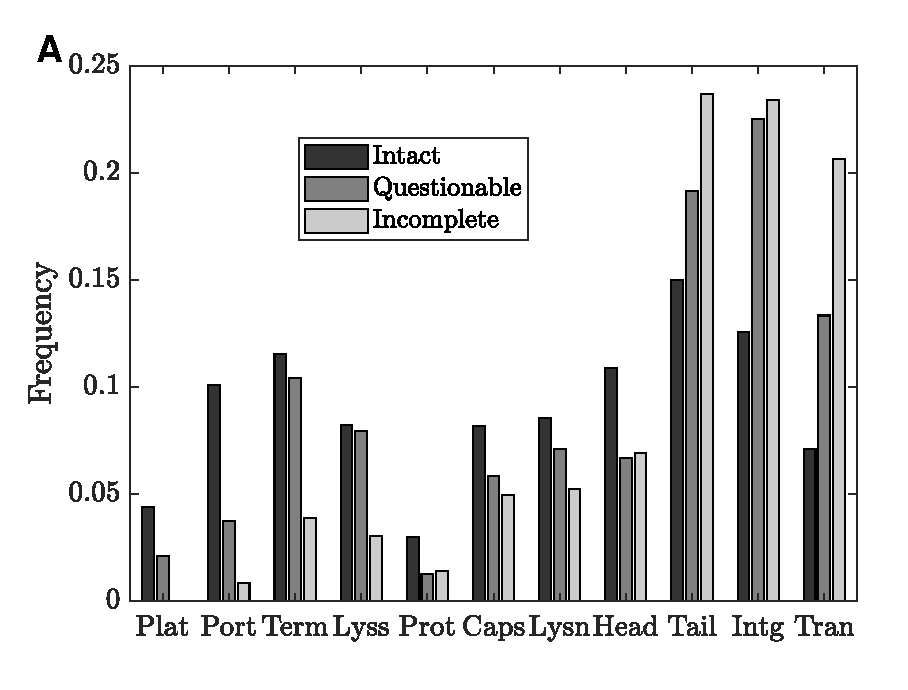
\includegraphics[scale=0.50]{bobay1}
     \end{subfigure}\hfill
     \begin{subfigure}[t]{0.50\textwidth} 
    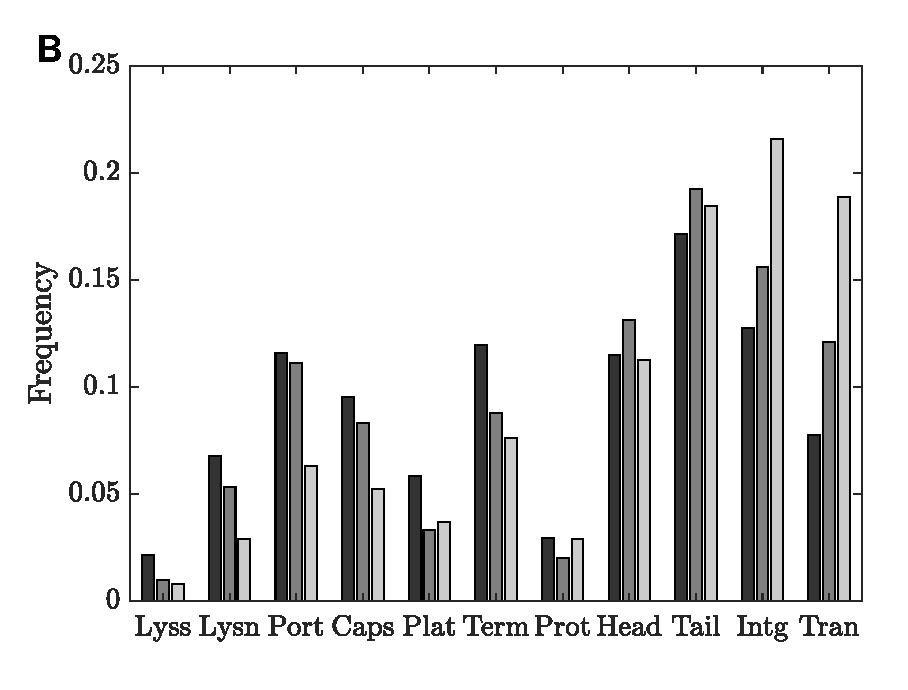
\includegraphics[scale=0.50]{aclame1}
    \end{subfigure}\hfill
         \begin{subfigure}[t]{0.50\textwidth}
    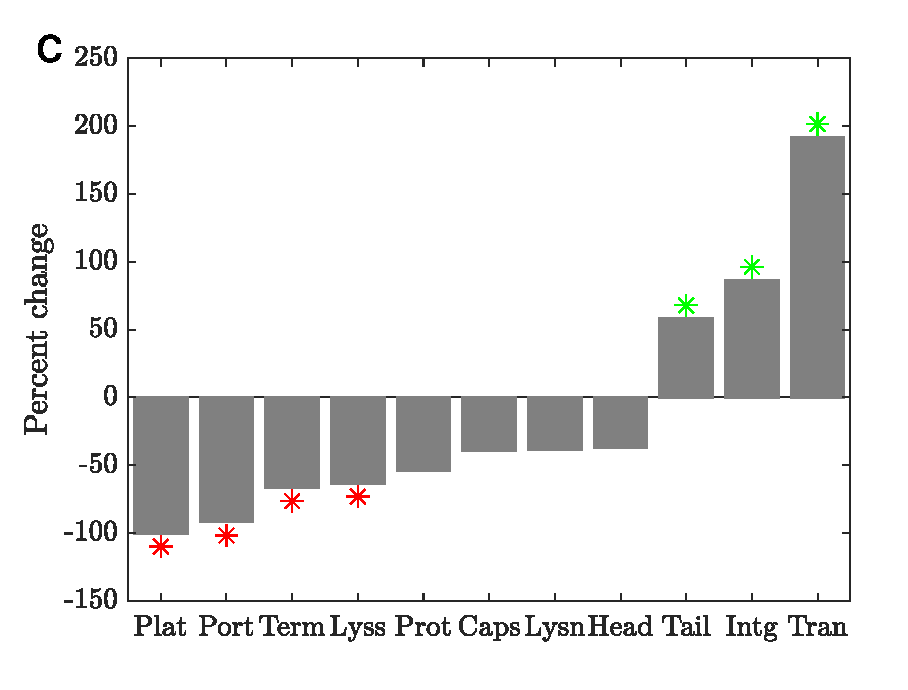
\includegraphics[scale=0.50]{bobay2}
     \end{subfigure}\hfill
     \begin{subfigure}[t]{0.50\textwidth} 
    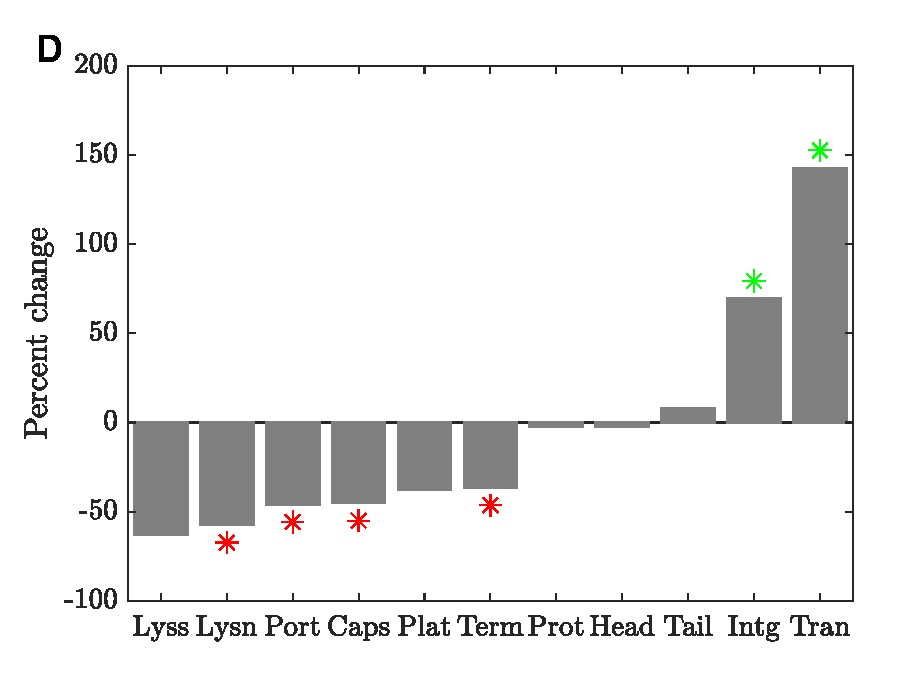
\includegraphics[scale=0.50]{aclame2}
     \end{subfigure}\hfill
    \caption[Changes in prophage gene frequencies, for intact, questionable and incomplete prophages.]{Changes in prophage gene frequencies, for intact, questionable and incomplete prophages.  (A) The frequency of each gene class identified in Table \ref{tab:genes} in prophages from Data Set 1 \cite{bobay_pervasive_2014}, for prophages identified as intact, questionable or incomplete.  Gene classes that constituted less than 1\% of the data have been excluded. Gene classes are ordered by the percent change in frequency (degree to which they are enriched in incomplete prophages, see panel C.) (B) Gene frequencies as in panel A, but for Data Set 2 \cite{leplae_aclame:_2010}.  (C) Percent change in gene frequency; the frequency of each gene class in incomplete prophages is compared to the baseline frequency of that class in intact prophages.  Frequencies that were significantly lower (red) or higher (green) than expected by chance with a two-sided 5\% significance threshold are indicated by stars.  Thus red stars indicate gene classes that are preferentially lost, while green stars indicate classes that are enriched in short prophages.  (D) Percent change in gene frequency for Data Set 2.} 
\label{fig:data4}
\end{figure}

To evaluate the statistical significance of these results, for each gene type we use the same number of identified genes (e.g. 317+25+14 = 356 for terminase in Data Set 1), and randomly assign the genes to one of the three prophage classes.  Because intact prophages in the dataset contain more genes than incomplete prophages, we also preserve the proportion of genes assigned to each class.  Thus in randomly assigning genes to prophage classes, we assign 2752/(2752+240+363) = 82\% of genes to intact prophages in Data Set 1, for example, while only
363/(2752+240+363) = 11\% are assigned to
incomplete prophages.

We computed the percent change in gene frequency for these bootstrapped data as described above, and repeated this procedure 10,000 times.  Stars in the lower panels of Figure \ref{fig:data4} indicate \% change values in the data that were lower than the 2.5 percentile or higher than the 97.5 percentile in the bootstrapped distributions.

These results reveal several features that are conserved between data sets.  We note that lysis or lysin genes, as well as portal and terminase proteins, are preferentially lost in incomplete prophages.  In contrast, transposase and integrase genes are substantially enriched.  We explore these results further in both the computational and mathematical models described in the sections to follow.

In light of the striking enrichment of transposase genes in incomplete prophages, we examined the transposase annotations in greater detail.  For each prophage in the dataset, we downloaded the coding sequences and the BLAST hits identified for each coding sequence by PHASTER \cite{arndt_phaster:_2016}.  We counted the number of coding sequences with a BLAST hit annotated as an insertion sequence (IS) transposase (e.g. ``IS3 transposase B''), as well as those annotated as a transposase but without a BLAST hit to an IS.  As a control, we also counted the total number of proteins identified as a ``phage hit protein'' by PHASTER in each data set.  

As shown in Table \ref{tab:transp}, IS transposases account for 41.4\% of the transposase sequences identified in Data Set 1, and 49.8\% of those in Data Set 2.  In Data Set 1, the frequency of IS transposases (calculated as the fraction of all phage proteins identified) is enriched 4.9-fold in incomplete prophages as compared to intact prophages; the frequency of non-IS transposases also increased but to a lesser degree (3.3-fold).  In Data Set 2, the frequency of IS transposases increased by 10\% in incomplete prophages, while non-IS transposases were reduced by 0.6\%.  Thus in both data sets, the frequency of IS transposases is enriched in incomplete prophages, and enriched to a greater degree than non-IS transposases.  As discussed further below, this suggests that the enrichment of transposase sequences in incomplete prophages may be due to the disruption of essential prophage functions due to IS insertion; in other words, the presence of the IS transposase has rendered the prophage cryptic.


\section{Analytical model of prophage gene content}

To investigate the preferential loss or maintenance of specific classes of phage genes in prophage sequences over time, we developed a mathematical model.  The model, although simplified, allows us to predict the effects of key parameters on the longterm genetic repertoire of prophages.

The model tracks a population of bacterial genomes, which contain prophages with genes in three possible types -- beneficial genes, excision genes and re-infection genes. Beneficial genes are genes that confer a selective advantage to the host, thus increasing the prophage population through vertical transmission. Biological examples of beneficial genes include host virulence factors that help the bacterial cell during colonization of its host (for example phage lambda's \emph{lom} gene). In contrast, excision genes are the genes involved in prophage induction into the lytic cycle, which leads to the death of the host cell. Examples of excision genes include lambda's \emph{O} and \emph{P} genes, which switch on the lytic cycle by commandeering the host's DNA polymerase. Phage induction will typically lead to bacterial cell death regardless of the quantity or quality of phage progeny.  Phage progeny success is determined by the phage's re-infection genes, comprising the genes required for phage genome replication, packaging, lysis, transmission to a new host, and reestablishment of lysogeny.  This re-infection class, in particular, includes a large number of genes of different function; yet their net effect, taken together, is to increase the prophage population through horizontal transmission.



In the simplified model, we consider a full prophage as one containing just three `genes', one of each class.  Here, we can think of a `gene' as a full functional complement of the underlying sequences required for each function.  We denote the frequency of full prophages in the population at time $t$ as $P_{1 1 1}(t)$. More generally, we use the notation $P_{ber}$ to represent the frequency of prophages with (1) or without (0) the beneficial, excision or re-infection genes respectively.  For completeness, the model also includes a population $P_{000}$ corresponding to bacterial genomes in which the prophage has been completely lost.  Note that in the computational model to follow, we will both expand these gene classes and include multiple genes per class.

The analytical model includes the following processes:

{\bf Degradation}:  Each gene in each prophage in the population is lost (gene deletion) at rate $r_{D}$. For example, the frequency of $P_{111}$ is lost at overall rate $3r_D$, contributing at rate $r_D$ to each of the populations $P_{011}$, $P_{101}$ and $P_{110}$.

{\bf Induction}: If a bacterial genome contains a prophage which carries the excision gene, the prophage induces at rate $r_I$ and the bacterium is lost from the population.

{\bf Re-infection}:  Prophages that carry both the excision and re-infection genes ($P_{111}$ and $P_{011}$) reproduce (create copies of themselves in new bacterial genomes), through lysis, re-infection and lysogeny, at rate $r_L$.  %Note that in the mathematical model, new (full length) prophages are not added to the prophage population from an external pool.
    
{\bf Selection}: To model the potential selective benefit conferred by the prophage, we assume that bacterial populations that carry the beneficial prophage gene grow at per capita rate $r_S$.

These assumptions yield the following system of ordinary differential equations, illustrated as a schematic in Figure \ref{fig:schematic}:

\begin{eqnarray}
\frac{d P_{1\,1\, 1}}{dt} &=& (r_L  +r_{S} - 3 r_{D} - r_{I}) P_{1\,1\, 1} - \phi P_{1\,1\,1} \nonumber\\
\frac{d P_{0\,1\, 1}}{dt} &=& (r_L - 2 r_{D} - r_{I}) P_{0\,1\, 1}+ r_{D}P_{1\, 1\, 1} - \phi P_{0\,1\,1}  \nonumber\\
\frac{d P_{1\,0\, 1}}{dt} &=& (r_{S} - 2 r_{D}) P_{1\,0\, 1} + r_D P_{1\,1\, 1}- \phi P_{1\,0\,1} \nonumber\\
\frac{d P_{1\,1\, 0}}{dt} &=& (r_{S} - 2 r_{D} - r_{I}) P_{1\,1\, 0}+ r_{D} P_{1\,1\, 1} - \phi P_{1\,1\,0}  \nonumber\\
\frac{d P_{0\,0\, 1}}{dt} &=& (- r_{D}) P_{0\,0\, 1} + r_{D} P_{0\,1\, 1} +r_{D} P_{1\,0\, 1}- \phi P_{0\,0\,1} \nonumber\\
\frac{d P_{0\,1\, 0}}{dt} &=& (- r_{D} - r_{I}) P_{0\,1\, 0} + r_{D} P_{0\,1\, 1} +r_{D} P_{1\,1\, 0}- \phi P_{0\,1\,0} \nonumber\\
\frac{d P_{1\,0\, 0}}{dt} &=& (r_{S} - r_{D}) P_{1\,0\, 0}+ r_{D} P_{1\,0\, 1} +r_{D} P_{1\,1\, 0}- \phi P_{1\,0\,0}\nonumber\\
\frac{d P_{0\,0\, 0}}{dt} &=&  r_{D}( P_{1\,0\, 0} + P_{0\,1\, 0} + P_{0\,0\,1})
- \phi P_{0\,0\,0}\,\,.
\label{systemC}
\end{eqnarray} 
Here, terms involving $\phi$ simply ensure that the frequencies sum to unity at all times, with $\phi$ defined as:
\[\phi = (r_L  +r_{S} - r_{I}) P_{1\,1\, 1} +  (r_L - r_{I}) P_{0\,1\, 1} + r_{S} P_{1\,0\, 1} + (r_{S}- r_{I}) P_{1\,1\, 0} - r_{I} P_{0\,1\, 0} + r_{S} P_{1\,0\, 0}\,\,.
\]

\begin{figure}[H]
 \centering
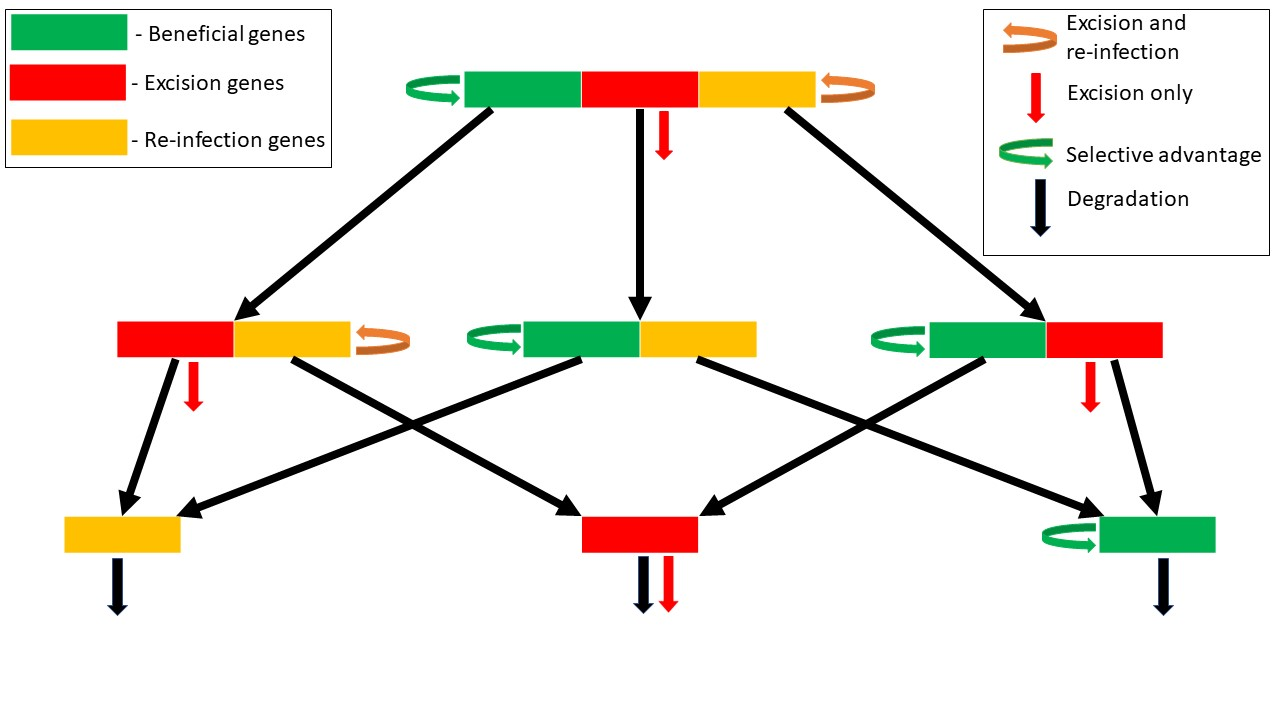
\includegraphics[width=15cm]{Model}
\caption{Schematic diagram of the mathematical model.}
\label{fig:schematic}
\end{figure}

A detailed analysis of the equilibria and stability of this 8-dimensional model is provided in the Supplementary Material. From this analysis, we find four possible longterm outcomes: (1) equilibrium $E_0$, in which all prophage genes are lost; (2) equilibrium $E_B$, in which both excision and re-infection genes are lost, but beneficial genes persist.  This equilibrium reflects complete domestication of the prophage; (3) equilibrium $E_{ER}$, in which beneficial genes are lost but both excision and re-infection genes persist. This corresponds to a virulent prophage that does not contribute to host fitness; (4) equilibrium $E_A$, in which all three types of genes persist.

As described in the Supplementary Material, two critical conditions are sufficient to determine the long-term behaviour of the prophage gene distribution.

Condition 1: $r_S> r_D$. Note that $r_S$ is the rate at which a beneficial gene produces a new copy of itself, while $r_D$ is the rate at which a beneficial gene is lost, which occurs through mutational degradation.  Thus $r_S>r_D$ implies that on average, a beneficial gene makes more than one copy of itself before it is lost: beneficial genes persist.

Condition 2: $r_L> 2r_D + r_I$.  Similarly, the combination of an excision and a re-infection gene, co-occuring on a prophage, is able to produce a new copy of itself at rate $r_L$. These genes may be lost through induction, but also lost if either gene is degraded by mutation, so the total rate of loss is $2r_D + r_I$.  Thus this gene combination can persist if $r_L>2r_D + r_I$.

The predicted behaviour of the mathematical model can therefore be summarized as shown in Table \ref{tab:conditions}.

\renewcommand{\baselinestretch}{1}
\begin{table}
\centering
\begin{tabular}{| c | c | c |}
\hline
{\bf Longterm prediction} & B genes do not persist & B genes persist \\
Condition & $r_S<r_D$ & $r_S > r_D$ \\
\hline
ER genes do not persist & {\bf extinction} &  {\bf domestication} \\
$r_L < 2r_D + r_I$ &  $E_0$ & $E_B$ \\
\hline
ER genes persist & {\bf virulence} & {\bf persistence} \\
$r_L > 2r_D + r_I$ &  $E_{ER}$ & $E_A$ \\
\hline
\end{tabular}
\caption{Conditions determining which classes of prophage genes persist longterm.}
\label{tab:conditions}
\end{table}
\renewcommand{\baselinestretch}{2}

In Figure \ref{fig:mathresults}, we illustrate the approach of System \ref{systemC} to each of these four equilibrium states, for appropriate parameter values.  To simplify the presentation, we plot the the average number of genes of each type carried per prophage, where for example the average number of beneficial genes per prophage is given by $P_{111} + P_{110} + P_{101} + P_{100}$.  Equivalently, this is the fraction of prophages that carry the beneficial gene.

 \begin{figure}[H]
    \centering
     \begin{subfigure}[t]{0.50\textwidth} 
    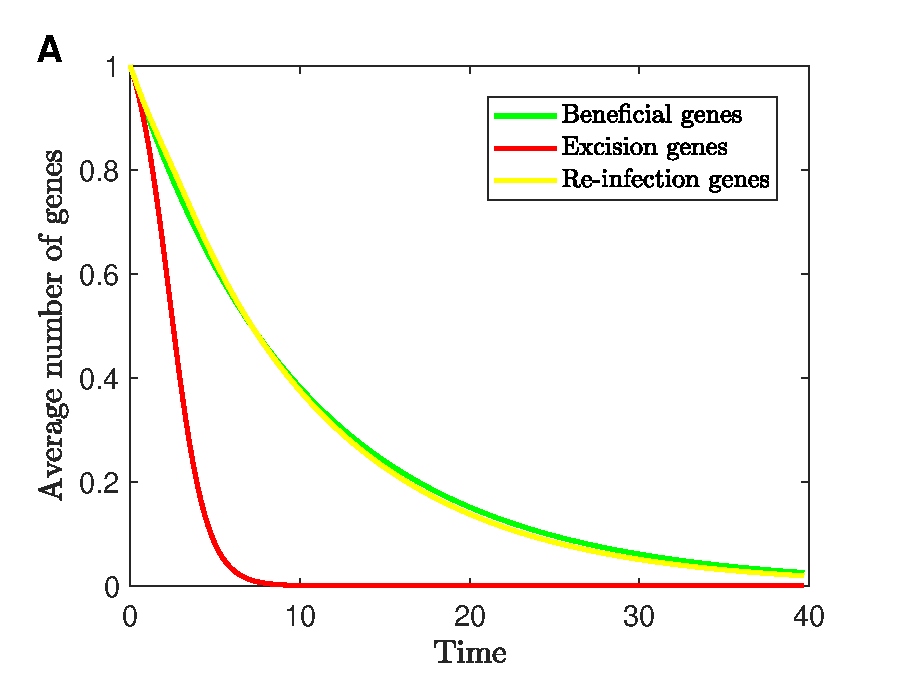
\includegraphics[scale=0.50]{triv}
     \end{subfigure}\hfill
         \begin{subfigure}[t]{0.50\textwidth}
    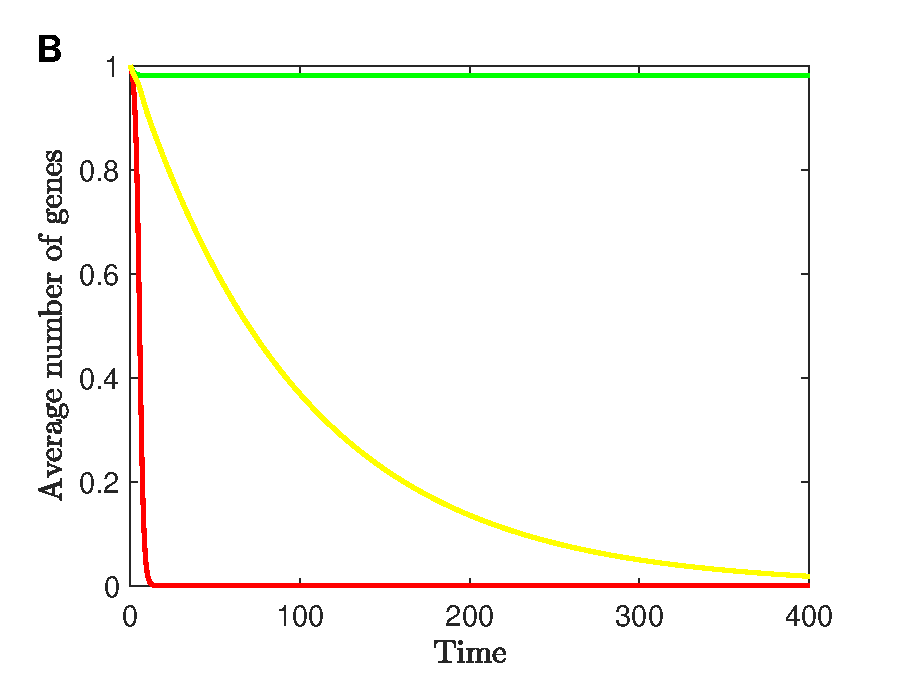
\includegraphics[scale=0.50]{E_b}
    \end{subfigure}\hfill\\  \begin{subfigure}[t]{0.50\textwidth}
        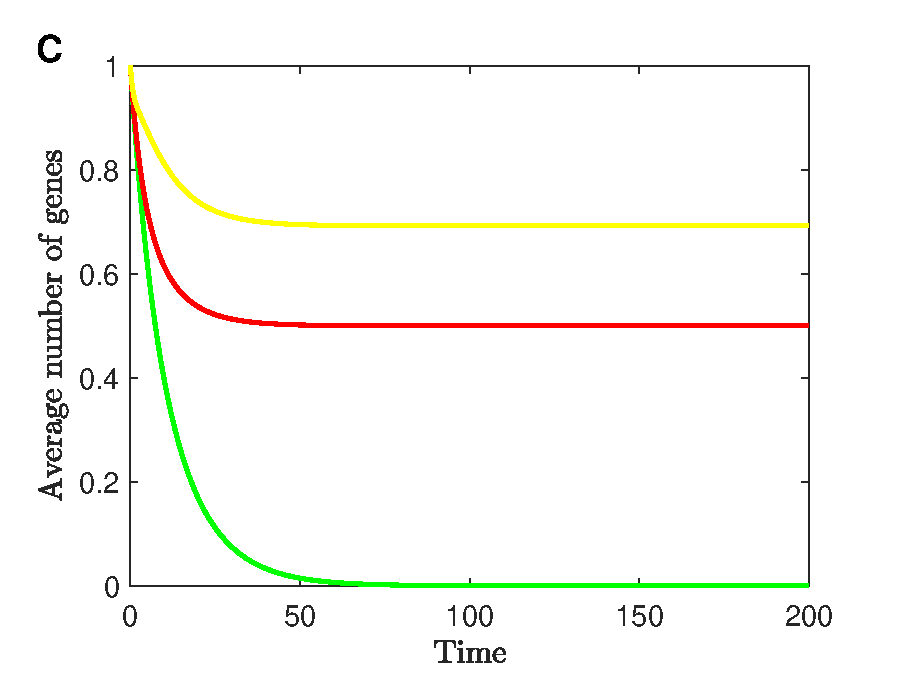
\includegraphics[scale=0.50]{E_li}
    \end{subfigure}\hfill   \begin{subfigure}[t]{0.50\textwidth}
    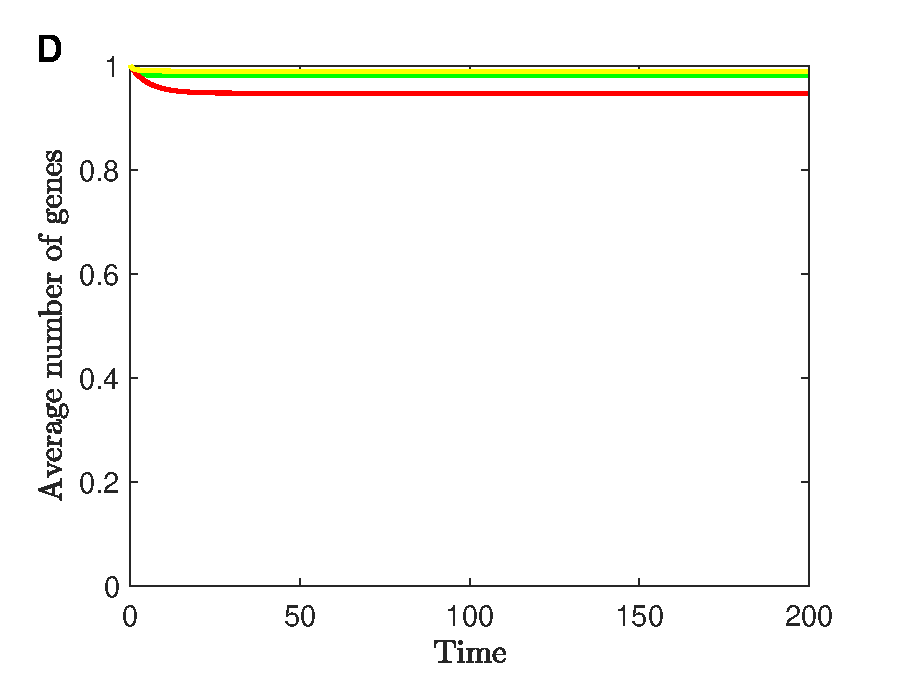
\includegraphics[scale=0.50]{E_lib}
    \end{subfigure} 
     \caption[Numerical integration of the analytical model.]{Numerical integration of the analytical model, showing System \ref{systemC} converging toward four possible equilibria: (A) {\bf Extinction}, $E_0$($r_S = 0.01 , \, r_D =0.1 , \, r_L =0.2 \, $);  (B) {\bf Domestication}, $E_B$ ($r_S = 0.52 , \, r_D =0.01 , \, r_L =0.2  $); (C) {\bf Virulence}, $E_{ER}$ ($r_S = 0.02 , \, r_D =0.1 , \, r_L =1.3  \, $); (D) {\bf Persistence}, $E_A$ ($r_S = 0.52 , \, r_D =0.01 , \, r_L =1.2  \, $).  In all cases, $r_I=1$.}
     \label{fig:mathresults}
     \end{figure}
\section{Gene Repertoire Simulations}

We also developed a computational model which is able to describe the gene content of prophage sequences in greater detail.  Here, we assume that prophages exist in a population of bacterial genomes that are linked by both cellular reproduction (vertical transmission of the prophage) and horizontal gene transfer (horizontal transmission).  We can vary the initial conditions such that all or only some of the bacterial genomes initially carry prophages.  Bacterial genomes that carry inducible prophage sequences may be lost through induction and lysis, whereas bacterial genomes that carry beneficial prophage sequences may be preferentially copied to the next generation.  We describe these steps in detail below.

Each prophage sequence may contain genes of the following four types: excision genes, re-infection genes, beneficial genes and neutral genes.  A full prophage carries $n_E$ excision genes, $n_R$ re-infection genes, $n_B$ beneficial and $n_N$ neutral genes.  We include mutational degradation and also include the possibility that an insertion sequence (or other transposable element) could disrupt the prophage genome. 

We track the presence or absence of each gene in each prophage sequence. A discrete timestep in the simulation corresponds to a bacterial generation time.  The rates of the underlying processes, however, are expressed in units of the ``prophage generation time", that is, the average time that a single prophage sequence is maintained in a bacterial genome before induction \cite{khan_quantifying_2019}.  Since the bacterial generation time, $\Delta t$, is much shorter than the prophage generation time, if a process occurs at rate $r$ per prophage generation, the probability that it occurs in timestep $\Delta t$ is small and well-approximated by $r \Delta t$.

The following processes are included in the model, with parameters as described in Table \ref{tab:params}:

{\bf Degradation}:  In each time step, each gene in each prophage in the population is removed (gene deletion) with probability $r_{D} \Delta t $. 

{\bf Induction}: If a prophage carries all $n_E$ excision genes, it may induce with probability $r_I \Delta t$.  When a prophage induces, it is removed from the population.  We thus assume that all $n_E$ excision genes are required for excision and death of the host cell.  Note that we ignore polylysogeny, that is, we make the simplifying assumption that excision and cell death affect only the excising prophage.

{\bf Re-Infection}:  To simulate the process of lysis followed by re-infection and lysogeny, a copy of any prophages that carry all $n_E$ excision genes \emph{and} all $n_R$ re-infection genes may be added to the prophage pool with probability $r_L \Delta t$.
Thus, full complements of both the excision and re-infection genes are required to reinfect.
In addition, in some simulations new (full length) prophages are added to the prophage pool with probability $r_F \Delta t$.  This might occur for example if there is an influx of prophages to the local population from an external pool.
    
{\bf Selection}: Copies of existing prophages are also added to the population at rate $r_S \Delta t\,n_b/n_B$.  Here $n_b$ is the number of beneficial genes carried by the prophage, and $r_S$ is the maximum selective benefit provided to the host cell if the prophage contains all $n_B$ beneficial genes. 

{\bf Population regulation}: We consider a pool of prophages that exists within a bacterial population that cannot grow unbounded.  To regulate the population size, if the current population size $N$, is greater than the bacterial carrying capacity, $K$, each bacterial genome is copied into the subsequent generation with probability $K/N$.
    
While all of our simulation studies include the processes described above, in some simulations we also explored the impact of disruption by transposable elements (TEs, such as bacterial insertion sequences) as follows.

{\bf TE disruption}: Motivated by the observed frequencies of IS transposase sequences in incomplete prophages, we include the possibility of TE disruptions in prophage genes.  For each gene in each timestep, a TE disruption may occur with probability $r_T \Delta t$.  When this occurs, we assume that gene function has been disrupted: if a beneficial gene has been disrupted, the gene confers no benefit to the host thereafter; if a gene required for excision or re-infection is disrupted, the prophage is no longer able to kill the host or re-infect respectively.  Thus TE disruptions have the same effect as gene deletions, but leave a signature of TE sequences in the prophage genome.  

We wondered whether it was reasonable to include TE disruptions in the model, since their rates might be negligible relative to mutational degradation. Rates of base pair substitutions in {\it E. coli} K12 have been estimated to be on the order of $2\times10^{-10}$ per nucleotide, per generation \cite{foster_determinants_2015}.  Multiplying by 1.2 kb per prophage gene \cite{khan_quantifying_2019} yields an estimate of $2.4\times10^{-7}$ base pair substitutions, per prophage gene, per bacterial generation.  Presumably only a fraction of base pair substitutions result in loss of function.  In addition, small indels are estimated to occur at about one tenth of this rate \cite{foster_determinants_2015}.  Thus taking in {\it E. coli} as a model organism, rates of prophage gene degradation through mutation (base pair substitution and short indels) might occur on the order of $10^{-7}$ or $10^{-8}$ per gene per generation.

In comparison, rates of transposition, for 5 insertion sequences in {\it E. coli} K12, have been estimated to be about $1\times10^{-5}$ per element per generation \cite{sousa_rates_2013}; this includes both copy-and-paste and cut-and-paste transpositions.  The ancestral genome in this mutation accumulation study carried a total of 33 copies of these ISs, yielding an overall transposition rate of $3.3\times10^{-4}$ transpositions per generation.  Given that a typical prophage gene comprises 1.2 kb \cite{khan_quantifying_2019} of a 4.6 Mb {\it E. coli} genome, we arrive at an estimated transposition rate of $8.6\times10^{-8}$ per prophage gene, per bacterial generation, similar to our estimate for gene loss through mutational degradation.

\begin{table}
\begin{tabular}{ p{2.5cm}p{11.5cm} }
\hline
Parameter   &  Description  \\
\hline
$n_B$ & number of beneficial genes\\
$n_E$ & number of genes necessary for excision\\
$n_R$ & number of genes necessary for re-infection\\
$n_N$ & number of neutral genes\\
$r_{D}$ & rate of loss through mutational degradation \\
$r_{I}$ & rate of loss through induction, excision and host death \\
$r_{L}$ & rate of increase through lysis, reinfection and lysogeny\\
$r_{T}$ & rate of loss through TE disruption\\
$r_S$ & selective advantage to host cell if prophage carries all beneficial genes  \\
\hline
\end{tabular}
\caption{Parameters of the computational model.}
\label{tab:params}
\end{table}

\subsection{Gene content of active temperate phage}

We used phage lambda's genome architecture as a model for the number of excision, beneficial, and reinfection genes in a temperate phage genome (see Figure 1 in \cite{rajagopala_protein_2011}). Lambda has long been a model system for the study of lytic-lysogeny cycles, phage genome arrangement, and phage evolution \cite{calendar_bacteriophages_2006}.

Excision genes: Lambda's excision genes are those that switch phage gene expression to the lytic cycle. Corresponding to the early right operon (6.5 kb), these excision genes make up approximately 13.3 percent of the phage genome.

Beneficial genes: Lambda carries several genes thought to confer benefit to the bacterial host during lysogeny. These include \emph{cI}, \emph{rexA}, \emph{rexB}, \emph{sieB}, \emph{lom}, and \emph{bor}, comprising ~3.7kb total, about 7.6 percent of the genome.

Reinfection genes: The rest of the lambda genome contains genes that allow a phage to form viable progeny capable of reinfecting other cells: phage particle production, packaging, lysis, and lysogeny. These genes include about 38.4 kb, ~79 percent of the genome. Most of these genes are contained in the late Operon (~27 kb, phage particle production) and the early left operon (~13 kb, lysogeny). The host-beneficial genes encoded in those operons (\emph{sieB}, \emph{lom}, \emph{bor}, ~1.6 kb total) are included instead in the beneficial genes category discussed above.

We note that not all lambda genes have been fully characterized. For example, lom and bor are thought to be host-beneficial during lysogeny, but more work is needed to establish the host fitness components. We also note that not all excision and reinfection phage genes are likely essential.

Taken together, these gene frequencies motivated the choice to model a full prophage genome in the ratio 1:1:8 for benefical:excision:re-infection genes.  In addition to these genes, in some simulations we also included neutral genes as a control. 
\subsection{Computational Model Results}
 Figure \ref{fig:simresults} illustrates that like the analytical model, the long-term behaviour of the simulation predicts four possible outcomes for the prophage: extinction, domestication, virulence (loss of genes that benefit the host but retention of genes necessary for virulent function) or persistence (of all gene types).  Although omitted for brevity, it is straightforward to derive conditions similar to those provided in Table \ref{tab:conditions} which predict the loss or retention of each gene type.  For example with 1 excision gene and 8 re-infection genes, the `ER' function can be lost by a mutation in any of these 9 genes, so the overall rate of loss is $9r_D + r_I$, while the rate of gain is $r_L$.
 \begin{figure}[hbt!]
    \centering
     \begin{subfigure}[t]{0.50\textwidth} 
    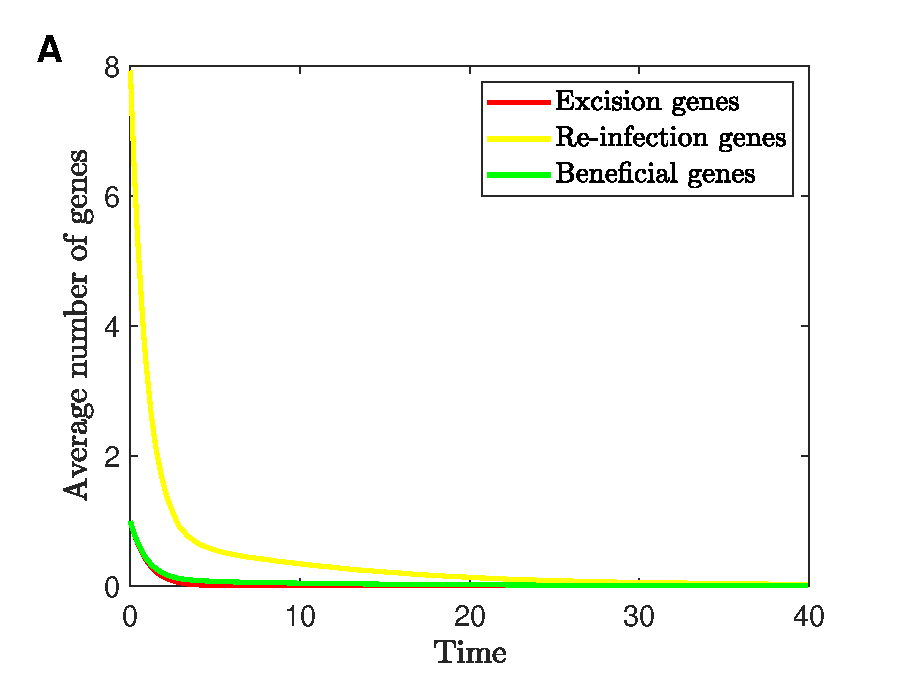
\includegraphics[scale=0.50]{trivSim1}
     \end{subfigure}\hfill
         \begin{subfigure}[t]{0.50\textwidth}
    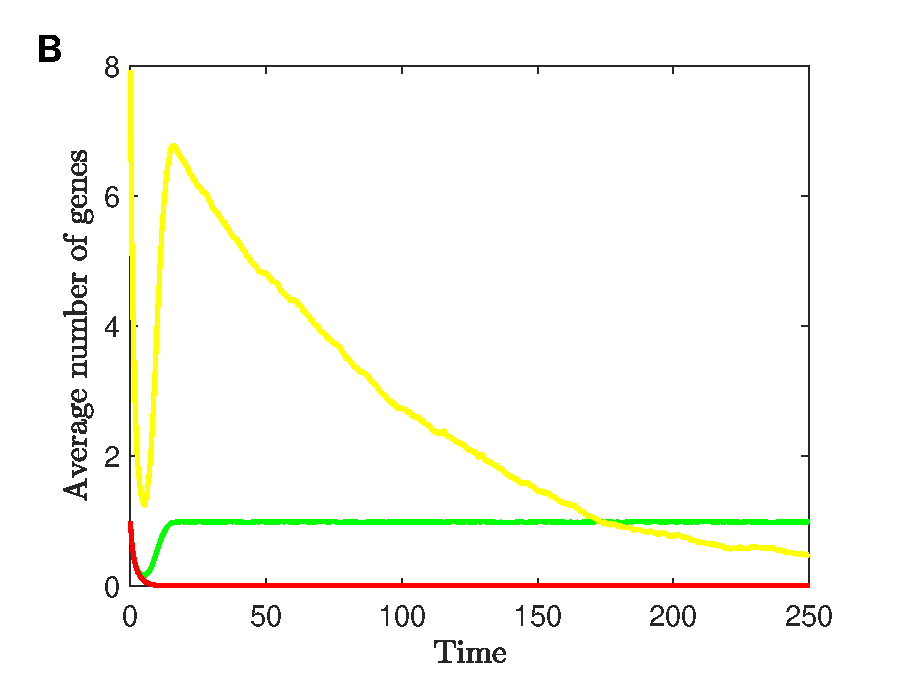
\includegraphics[scale=0.50]{E_bSim1}
    \end{subfigure}\hfill\\  \begin{subfigure}[t]{0.50\textwidth}
        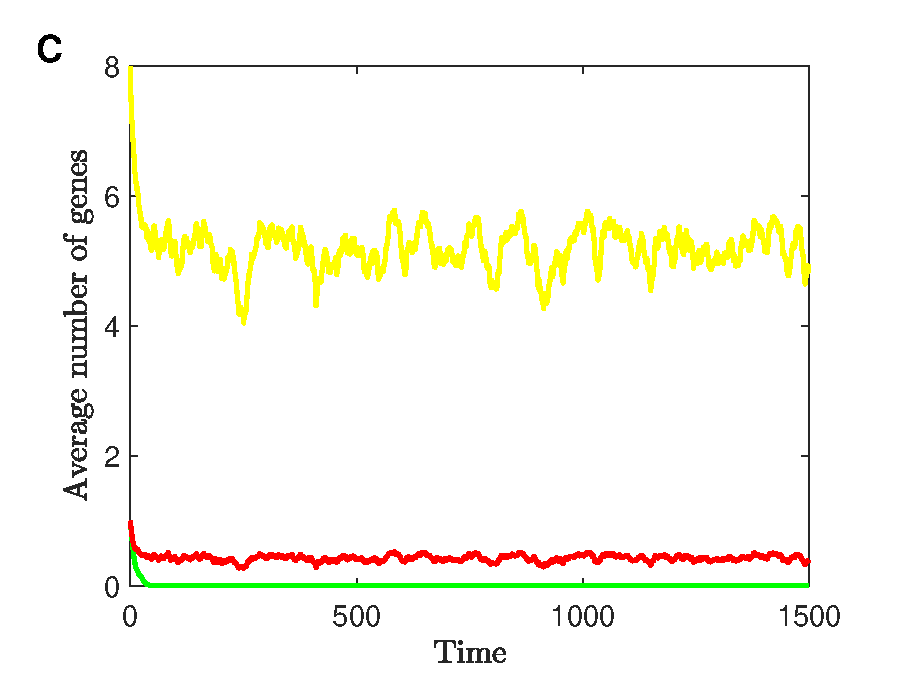
\includegraphics[scale=0.50]{E_liSim}
    \end{subfigure}\hfill   \begin{subfigure}[t]{0.50\textwidth}
    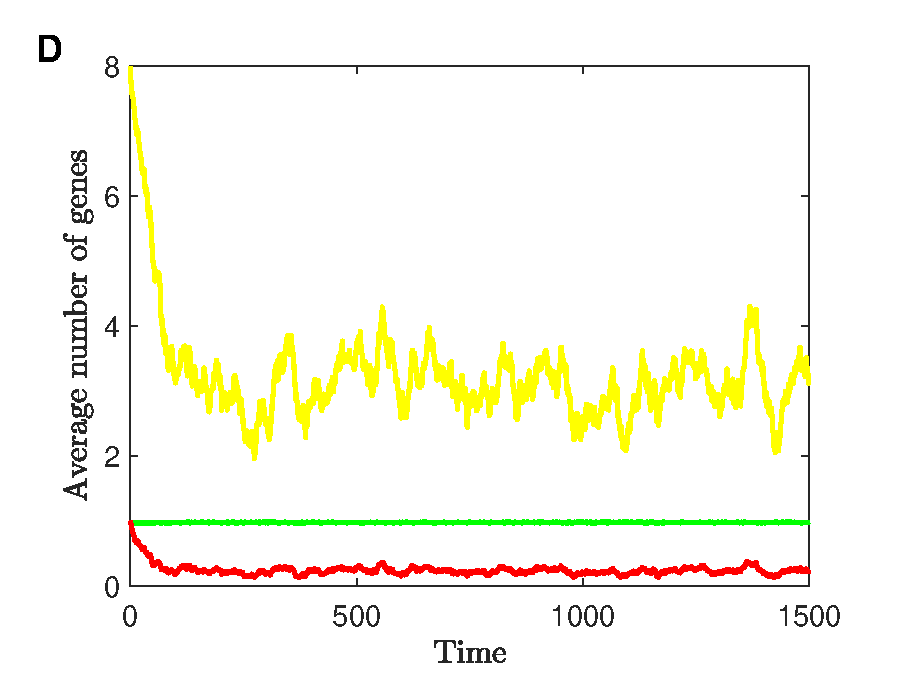
\includegraphics[scale=0.50]{E_libSim}
    \end{subfigure} 
     \caption[Simulations results showing the approach to four possible long-term outcomes.]{Simulations results showing the approach to four possible long-term outcomes:  (A) {\bf Extinction} ($r_S = 0.01 , \, r_D =0.1 , \, r_L =0.2 \, $);  (B) {\bf Domestication} ($r_S = 0.52 , \, r_D =0.01 , \, r_L =0.2  $); (C) {\bf Virulence} ($r_S = 0.02 , \, r_D =0.1 , \, r_L = 2.0  \, $); (D) {\bf Persistence} ($r_S = 1.5, \, r_D =0.05 , \, r_L =1.5  \, $).  In all cases, $r_I=1$, $r_T=0$, $n_B=1$, $n_E=1$ and $n_R=8$. The average number of genes of each type, per prophage, is plotted against time. }
     \label{fig:simresults}
     \end{figure}
 
  We further examined the qualitative features of the prophage population at the persistence equilibrium.  To do this, we  simulated the prophage population with parameter values as described in panel D of Figure \ref{fig:simresults} for 200 generations, and then compared the gene content of prophages of different lengths.  We define all prophages as either ``intact"  or ``incomplete": an intact prophage carries all the genes necessary for excision and re-infection, whereas if any of these genes is missing, the prophage is incomplete. Figure \ref{fig:Biresults}A shows the frequency of each type of gene in intact and incomplete prophages; the percent change in incomplete prophages, as compared to the baseline of an intact prophage, is shown in panel B.  We find that genes involved in excision and re-infection are preferentially lost in incomplete prophages.  
 
 These results are clarified in Figure \ref{fig:Biresults}C, which shows a histogram of prophage lengths (grey bars), along with the gene frequency for each gene type, for prophages of each length.  Thus for example full prophages have 10 genes and have 80\% re-infection genes, 10\% excision genes and 10\% beneficial genes.  We see a bimodal distribution of prophage lengths, with the smallest prophages becoming domesticated, that is, retaining only the gene that benefits the host.
 
  \begin{figure}[H]
    \centering
     \begin{subfigure}[t]{0.30\textwidth} 
    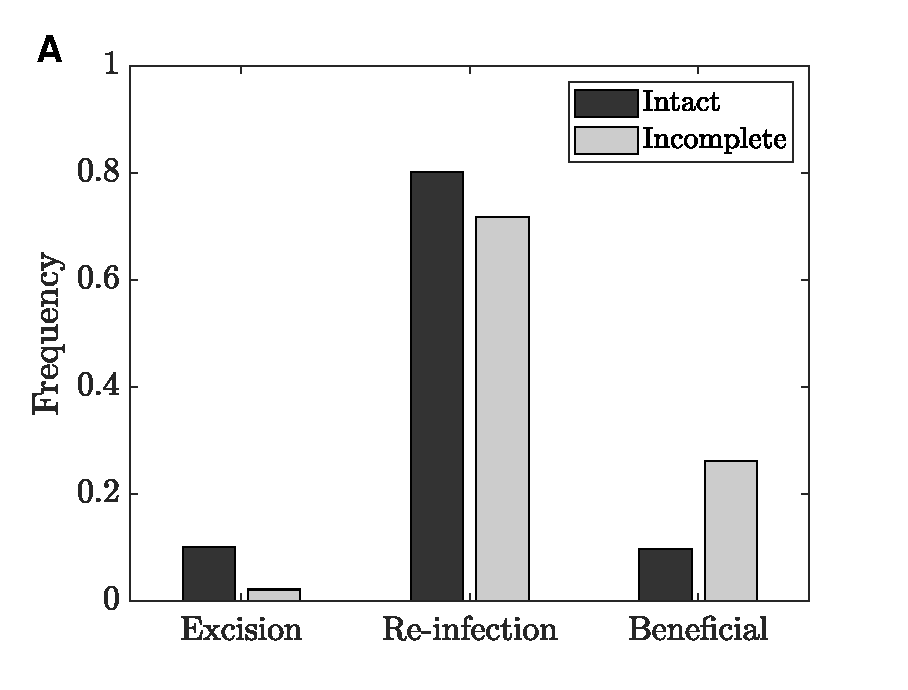
\includegraphics[height=1.8in,width=2.2in]{2Bi1}
     \end{subfigure}\hfill
         \begin{subfigure}[t]{0.30\textwidth}
    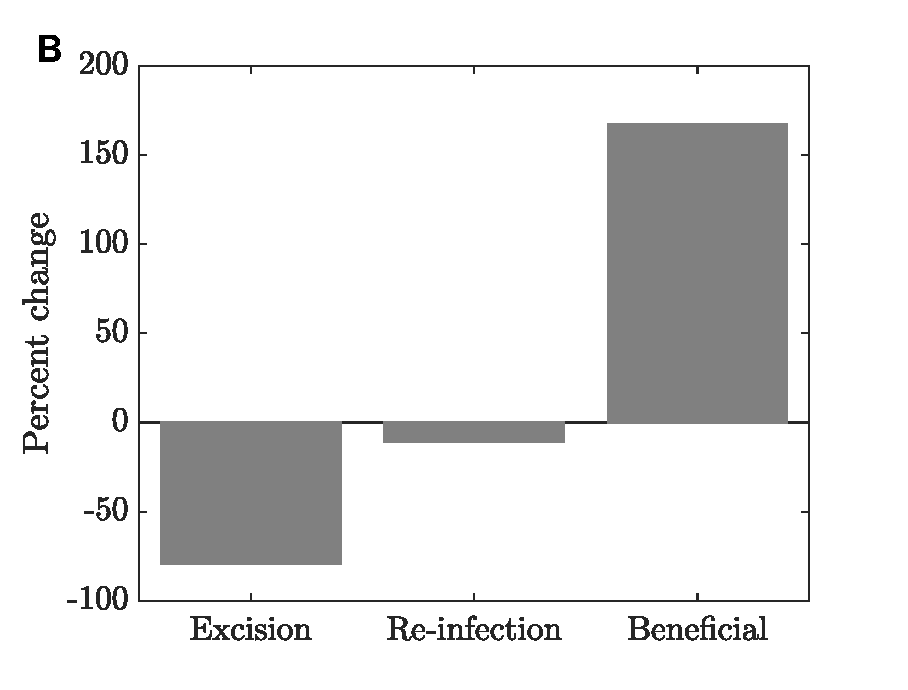
\includegraphics[height=1.8in,width=2.2in]{3Bi1}
    \end{subfigure}\hfill
    \begin{subfigure}[t]{0.30\textwidth}
        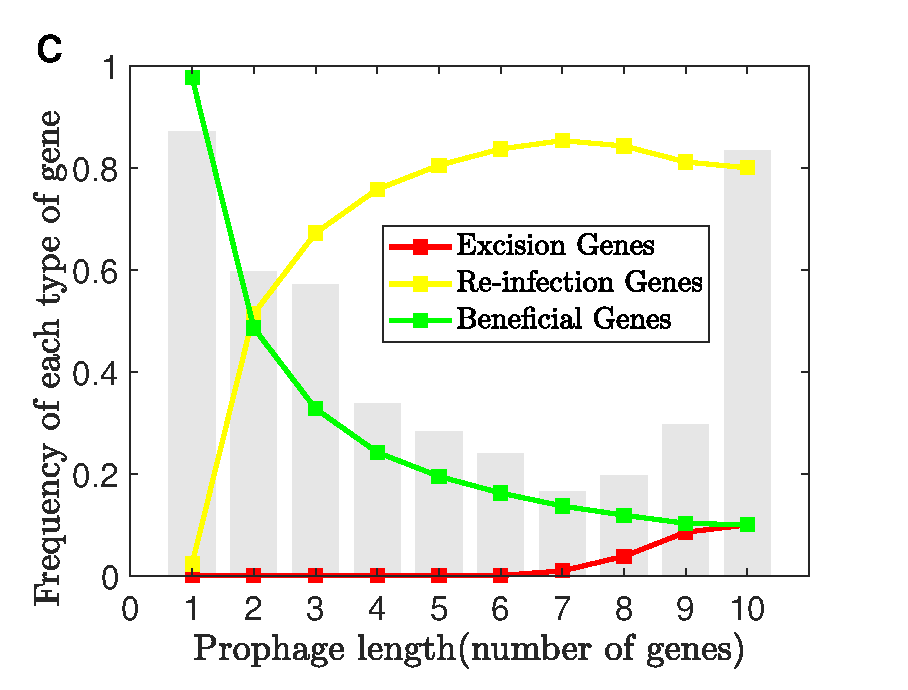
\includegraphics[height=1.8in,width=2.2in]{4Bi1}
    \end{subfigure}\hfill    
     \caption[Gene frequencies in intact and incomplete prophages.]{Gene frequencies in intact and incomplete prophages. (A) Frequency of genes of each type in intact and incomplete prophages, for the computational model simulated at the persistence equilibrium (see text for details); (B) Percent change in gene frequency from intact to incomplete; (C) A histogram of prophage lengths (grey bars), as well as the frequency of gene classes at each length.  We find a bimodal distribution of prophage sizes, with smaller prophages losing the excision and re-infection genes but retaining the beneficial gene.}
     \label{fig:Biresults}
     \end{figure}
     
 
 Fig. \ref{fig:TEsresults} illustrates the effect of adding transposable element disruptions to the computational model. In panel A, despite TE disruptions, the prophage population persists and retains all genes.  Here we have also added a single neutral gene, which has no effect on fitness, for comparison (grey line).  Panel D shows the average number of TE disruptions sustained in each type of gene; TEs accumulate in neutral genes but their presence in functional genes is minimized by purifying selection.  Panels B through F show similar results, except that the rate of TE disruption, $r_T$, and the selective advantage, $r_S$, are altered.  Increasing the transposition rate has the same qualitative effect as increasing the mutation rate, $r_D$, in Table \ref{tab:conditions}; the long-term outcome can change  from persistence (panel A) to either virulence (panel B) or domestication, depending on the value of $r_S$, and then ultimately to extinction (panel C) as $r_T$ increases.
 
 \begin{figure}[H]
    \centering
     \begin{subfigure}[t]{0.30\textwidth} 
    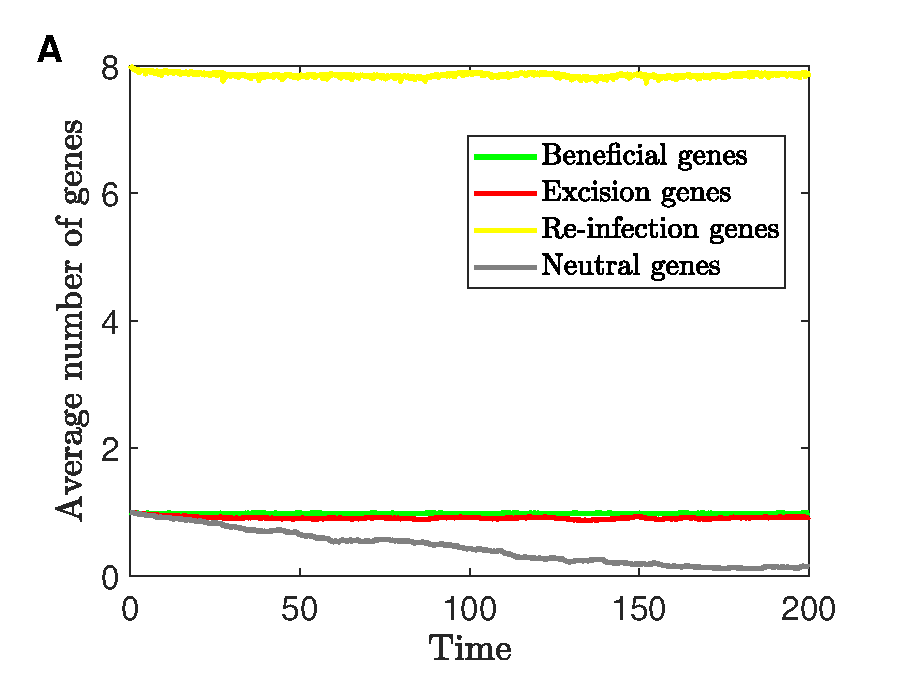
\includegraphics[height=1.8in,width=2.2in]{persisA}
     \end{subfigure}\hfill
         \begin{subfigure}[t]{0.30\textwidth}
    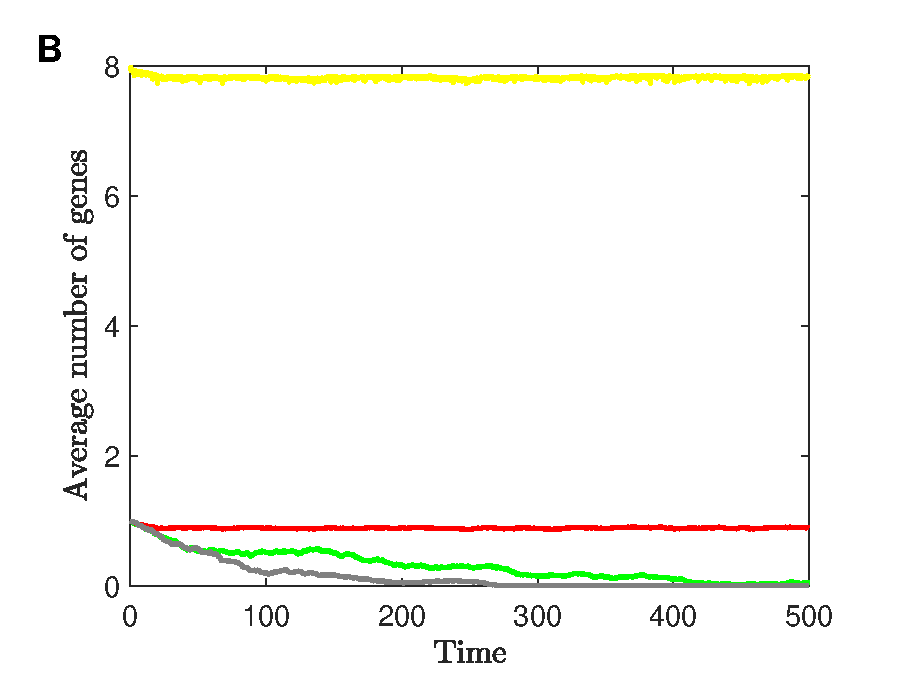
\includegraphics[height=1.8in,width=2.2in]{persisB}
    \end{subfigure}\hfill  
    \begin{subfigure}[t]{0.30\textwidth}
        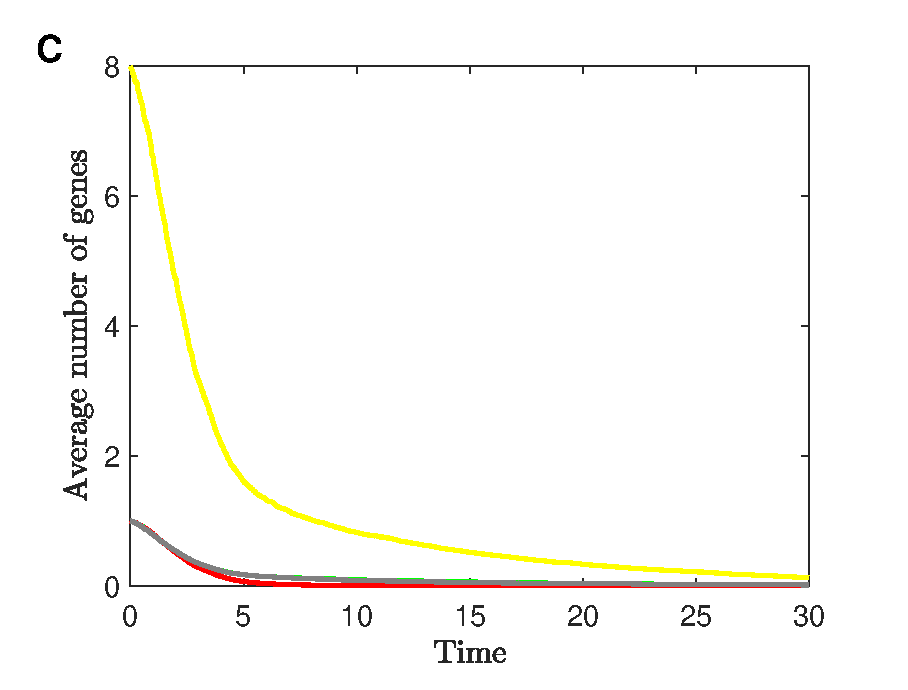
\includegraphics[height=1.8in,width=2.2in]{persisC}
    \end{subfigure}\hfill  \\  
      \begin{subfigure}[t]{0.30\textwidth} 
    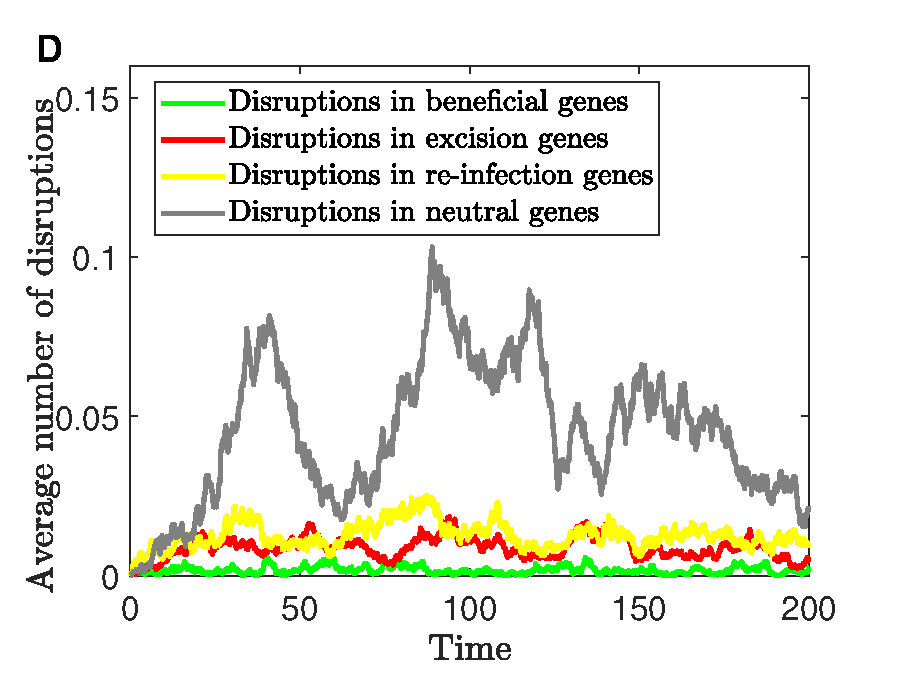
\includegraphics[height=1.8in,width=2.2in]{persisISD}
     \end{subfigure}\hfill
         \begin{subfigure}[t]{0.30\textwidth}
    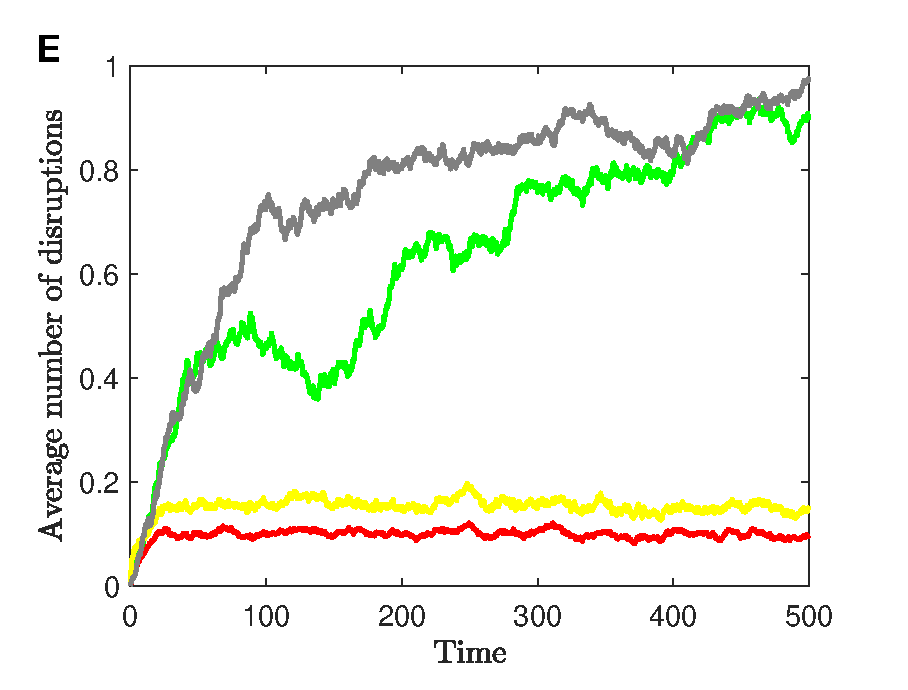
\includegraphics[height=1.8in,width=2.2in]{persisISE}
    \end{subfigure}\hfill
    \begin{subfigure}[t]{0.30\textwidth}
        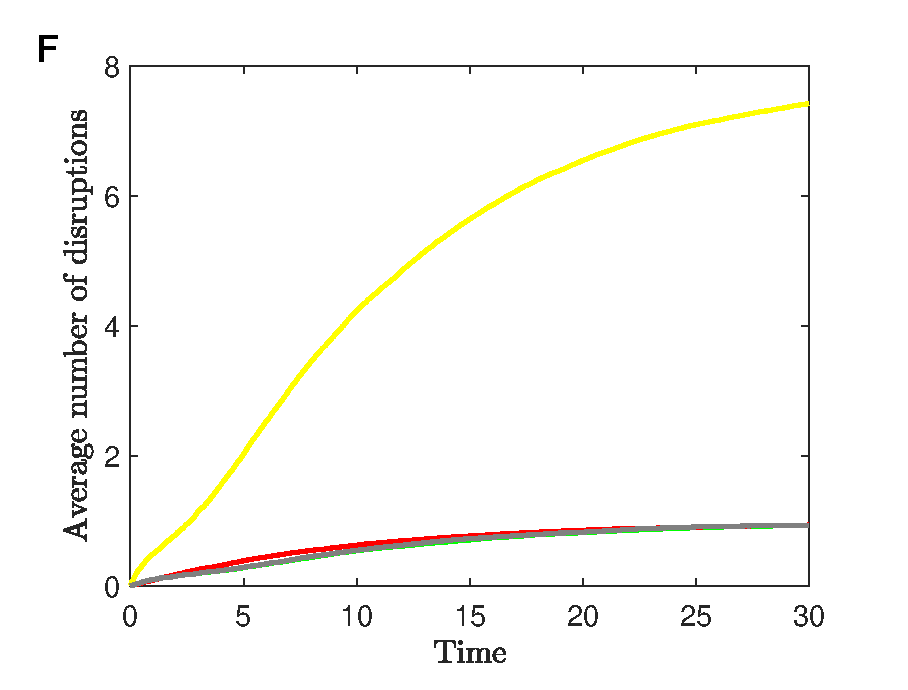
\includegraphics[height=1.8in,width=2.25in]{persisISF}
    \end{subfigure}\hfill  
     \caption[The effect of TE disruptions on the long-term outcome for prophage sequences]{The effect of TE disruptions on the long-term outcome for prophage sequences. In panels A through C, the average number of genes of each type per prophage is plotted against time.  As the transposition rate is increased, the long-term prediction for the prophage changes from persistence (panel A) to virulence (panel B) and finally to extinction (panel C).  Panels D through F show the average number of TE disruptions sustained in genes of each type versus time.  TEs accumulate in neutral genes but are limited in functional genes due to purifying selection.  Parameter values are:
     (A and D)  $r_S = 0.52, \, r_T = 0.009$;  (B and E) $r_S = 0.01, \, r_T = 0.01$; (C and F) $r_S = 0.002, \, r_T = 0.1$. In all cases, $r_I=1$, $r_L = 1.2$, $r_D = 0.001$, $n_B=1$, $n_E=1$, $n_R=8$ and $n_N=1$.}
     \label{fig:TEsresults}
     \end{figure}

Again, we simulated the prophage population with parameter values as described in panel D of Figure \ref{fig:simresults} for 5000 generations, but including TE disruptions ($r_T = 0.002$), comparing the gene content of intact and incomplete prophages.  Using the strict definition of ``intact"  or ``incomplete" described above, transposase genes were enriched nearly 400-fold in incomplete prophages (see Supplementary Material).  

This result may be artificially inflated by the fact that only the single beneficial gene can sustain a TE disruption in an intact prophage in our simulations.  In reality, algorithms such as PHASTER are not able to classify prophages as intact based on the certainty that they contain a full complement of functional phage genes.  Instead, approximate metrics are used, based for example on the number of identified phage genes in close proximity in the sequence \cite{arndt_phaster:_2016}. For a better comparison with the data shown in Figure \ref{fig:data4}, we therefore classified prophages as ``intact" if they contained 80\% of more of the possible prophage genes; prophages with less than 80\% were classified as incomplete.

Figure \ref{fig:Biresults80}A shows the frequency of each type of gene in intact and incomplete prophages classified in this way; the percent change in incomplete prophages, as compared to the baseline of an intact prophage, is shown in panel B.  Again we see that genes involved in excision and re-infection are preferentially lost, beneficial genes are preferentially maintained, and transposase genes are substantially enriched in shorter prophages.  

Figure \ref{fig:Biresults80}C shows a histogram of prophage lengths (grey bars), along with the gene frequency for each gene type, for prophages of each length.  A bimodal distribution of prophage lengths is again demonstrated, with the smallest prophages becoming domesticated, that is, retaining only the gene that benefits the host.  We note that transposase genes accumulate in prophages of intermediate length, but are absent from the smallest prophages.

  \begin{figure}[H]
    \centering
     \begin{subfigure}[t]{0.30\textwidth} 
    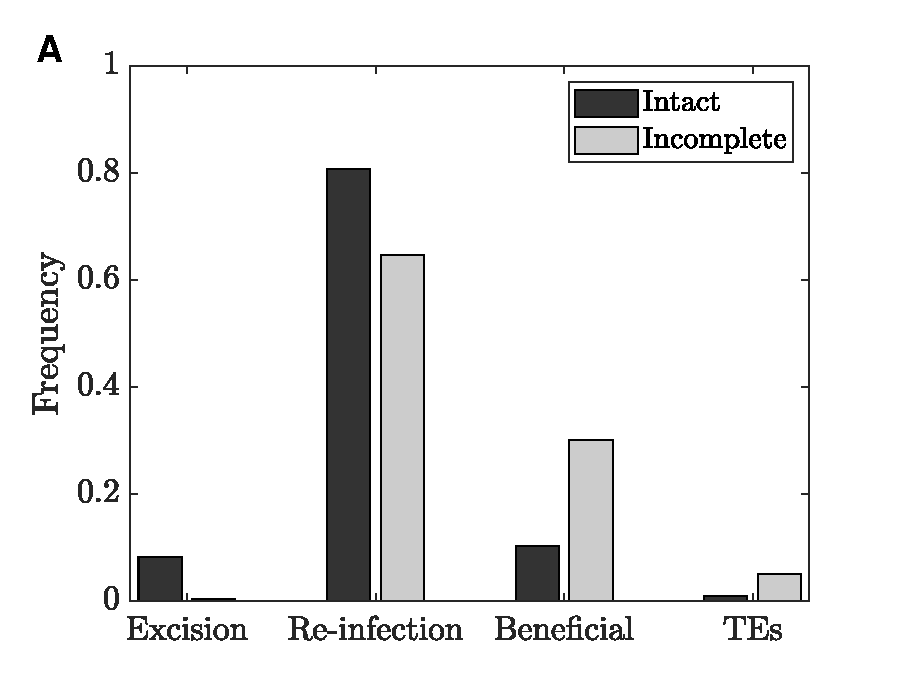
\includegraphics[height=1.8in,width=2.2in]{BiTe180}
     \end{subfigure}\hfill
         \begin{subfigure}[t]{0.30\textwidth}
    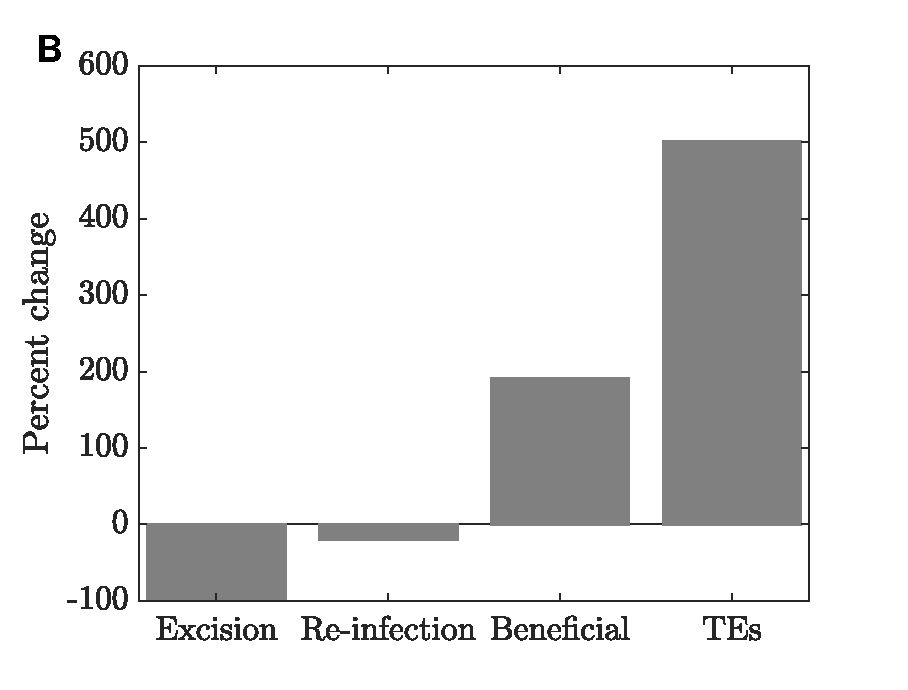
\includegraphics[height=1.8in,width=2.2in]{BiTe280}
    \end{subfigure}\hfill
    \begin{subfigure}[t]{0.30\textwidth}
        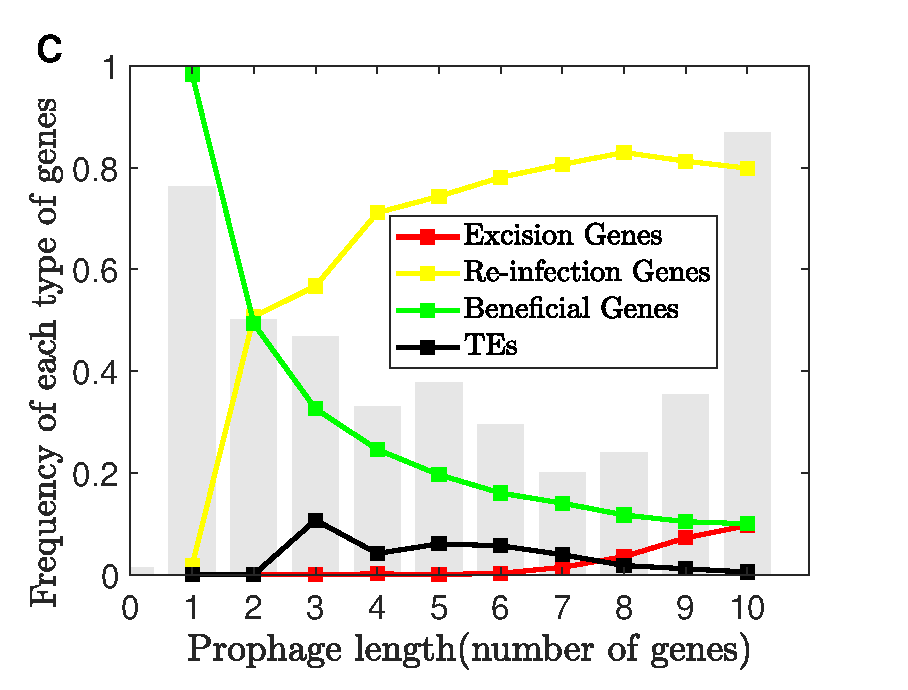
\includegraphics[height=1.8in,width=2.2in]{BiTe3o}
    \end{subfigure}\hfill    
     \caption[Gene frequencies in intact and incomplete prophages, when TEs are included.]{Gene frequencies in intact and incomplete prophages, when TEs are included ($r_S = 1.5, \, r_L = 1.5, \, r_D = 0.048, \, r_T = 0.002$). (A) Frequency of genes of each type in intact and incomplete prophages, for the computational model simulated at the persistence equilibrium with TE disruptions (see text for details); (B) Percent change in gene frequency from intact to incomplete; (C) A histogram of prophage lengths (grey bars), as well as the frequency of gene classes at each length.  We find a bimodal distribution of prophage sizes, with TEs accumulating in prophages of intermediate lengths.}
     \label{fig:Biresults80}
     \end{figure} 
 
 \section{Summary and Discussion}
 
 We bring three lines of evidence to bear on the diverse genetic repertoire of active and cryptic prophages.  First, we examine over 50,000 gene annotations from sequenced prophages to demonstrate that genes involved in lytic function -- structural genes such as plate, capsid and portal genes, as well as lysis, lysin and terminase genes -- are preferentially lost in incomplete (presumably cryptic) prophages.  In constrast, three gene classes are enriched: tail fiber, integrase and transposase genes (Fig. 1c, d).
 
 Secondly, a simplified mathematical model predicts that depending on the balance among dynamic processes such as the rates of lysis and infection, selection and mutational degradation, four longterm outcomes are predicted for prophage sequences: the maintenance of an active prophage that also carries host-beneficial genes, the maintenance of an active but virulent prophage, domestication, or extinction (Fig. 3 and Table 3).
 
 Thirdly, a more complex computational approach examines the genetic repertoires of prophages of differing lengths.  The computational model predicts a bimodal distribution of prophage lengths, as observed in a number of recent studies \cite{bobay_pervasive_2014, leplae_aclame:_2010, brueggemann_pneumococcal_2017, crispim_screening_2018}, and consistent with our recent predictions regarding the interplay of selection and mutation on the prophage length distribution \cite{khan_quantifying_2019}.  The computational model also demonstrates that genes involved in excision and re-infection are preferentially lost in shorter prophages (Fig. 5, 7), consistent with the loss of lytic-cycle specific genes observed our bioinformatic analyis (Fig. 1).  This result is intuitively appealing since selection at the level of the host favors loss of intact lytic-cycle alleles, which contribute to greater rates of host lysis and death.  
 
 As summarized above, our bioinformatic analysis supported a previous finding \cite{bobay_pervasive_2014} that some genes are significantly enriched in shorter prophages; in our data these enriched genes included transposases, phage tail protein-encoding genes, and integrases.  Consistent with these data, transposases preferentially accumulated in shorter prophages in our simulation studies, which assumed that transposable elements disrupted gene function and left an identifiable transposase gene sequence as a signature.
 
 Tail fibre genes, in contrast, would be classified as re-infection genes, and thus were not predicted to be enriched in cryptic prophages in our simulations.  Bobay et al. \cite{bobay_pervasive_2014} hypothesize that tail genes may be domesticated by bacterial hosts through the longer-term processes of co-option and evolution of novel function, for example the evolution of bacterial tailocin toxins from phage tail ancestors. For domestication of tail genes in this way, such processes would presumably require a specific combination of multiple accumulated mutations and the appropriate selective environment for a novel function to emerge. These conditions were well beyond the scope of our models here, but modeling the additional complexity of domestication via the accumulation of {\it de novo} adaptive mutations is an interesting idea for future work.
 
The enrichment of integrase genes in short prophages was an interesting and unexpected result of our bioinformatic analysis. Prophages typically possess integrase genes, facilitating chromosomal integration, and excision in conjugation with excisionase \cite{groth_phage_2004, casjens_prophages_2003,  frost_mobile_2005, ptashne_genetic_2004}. %Integrase genes typically mark one end of a prophage and are sufficiently conserved to be recognizable \cite{casjens_prophages_2003}.   
Prophage integrase genes have been used as recognized diagnostic markers for prophages within bacterial genomes \cite{ventura_prophage_2003,tran_sa3mw_2019}, as markers to identify temperate phage genomes \cite{song_prophage_2019}, and as signature genes to measure prophage diversity, and hence, host genome diversity \cite{colavecchio_prophage_2017}.
 %In this study the authors showed that food-associated isolates contain more integrase genes than clinical isolate. 
%1031 temperate phages out of 3540 phage genomes extracted from the NCBI
Based on these facts we were expecting that integrase genes may be missing in incomplete prophages (as suggested for example in \cite{colavecchio_prophage_2017}), yet the opposite trend was observed.

We suggest that integrase genes may be maintained through the evolution of phage-like genetic selfish elements, such as satellite phages and molecular parasites that don’t require the full complement of phage lytic cycle genes but benefit from horizontal transfer among hosts.  Integrase genes are commonly found on mobile genetic elements \cite{domingues_integrons:_2012}; when foreign DNA enters a host cell through horizontal transfer, integrase acts as a catalyst to mediate the process of recombination, thus integrases may facilitate the horizontal transfer of prophage-derived elements. The horizontal transmission of integrase genes along with their neighboring prophage genes would then result in significant enrichment of integrase genes in incomplete prophages.  Although our computational model has not yet incorporated horizontal transmission of full or partial prophages, this hypothesis could be explored more fully in an expanded model that includes horizontal gene transfer. 

 

\addcontentsline{toc}{chapter}{Bibliography}
\bibliographystyle{abbrv}
\bibliography{refrence} 


